\section{Statistical analysis}
\subsection{Confidence intervals and hypothesis tests}

\subsubsection{f)}
The sample was provided, data were took randomly from the population and they have been logged. It is possible to prove that they are identically normal distributed and we will do that at the end of this subsection. In this first part the data make no gender distinction. \\
The model is described by:
\begin{center}
$ X_i \sim N(\mu,\sigma^2) $ where $i=1,2,..,n$ \\
\end{center}
Hence we have 145 independent variables. \\
Our goal is to learn about the mean, the variance and the standard deviation of the population and find their precision. Using the already given values and taking the log of them we get:
\begin{table}[h]
\centering
\begin{tabular}{|c||c|c|c|c|}
  \hline
 \parbox{1.5cm}{\textbf{Variable} $BMI$} & \textbf{N. of obs.} & \parbox{1.5cm}{\textbf{Sample mean}} & \parbox{1.5cm}{\textbf{Sample var.}} & \parbox{1.5cm}{\textbf{Sample std. dev.}} \\
 \hline
  & $n$ & $(\overline{x})$ & $(s^2)$ & $(s)$ \\
  \hline
  \hline
Everyone & 145 & 3.218 & 0.1489 & 0.0222  \\ 
  \hline
\end{tabular}
\caption{Table with parameters of the model}
\label{Table2}
\end{table}
In order to perform model validation we have to look at different criteria such has: histograms and their shape, empirical c.d.f., Q-Q plot and wally plot. In this case we will use Q-Q plots and the wally plot. \\
Starting with two Q-Q plots in order: one with the normal values of BMI and the other with the logged values. It is already possible to see a bigger tendency to be normally distributed in the one where the logged values have been used \ref{logqq}. \\
\begin{figure}[h!]
    \centering
    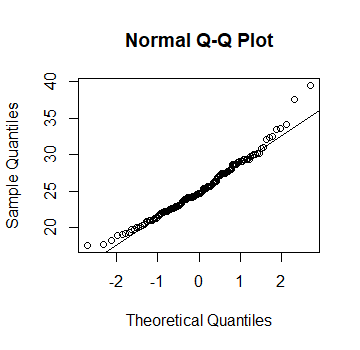
\includegraphics[scale=1]{root/Normal_q_q_plot.png}
    \caption{Q-Q plot of BMI scores}
    \label{normalqq}
    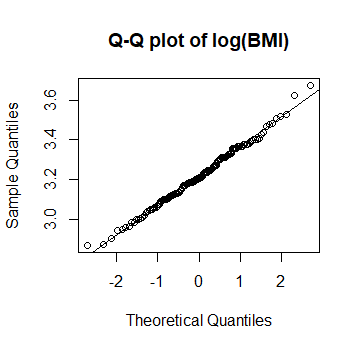
\includegraphics[scale=1]{root/q_q_plot_log.png}
    \caption{Q-Q plot of logged BMI scores}
    \label{logqq}
\end{figure}
\begin{figure}[h]
    \centering
    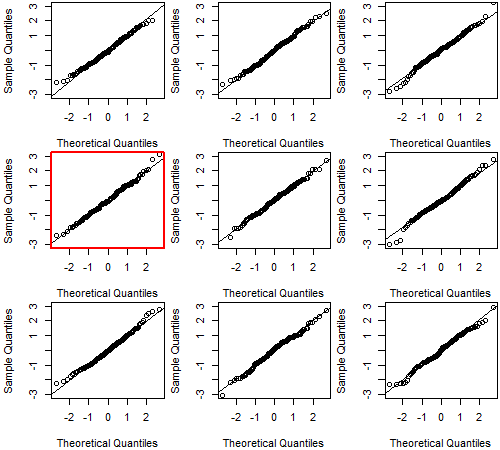
\includegraphics[scale=1]{root/Rplot.png}
    \caption{Wally plot of gender mixed data}
    \label{allWally}
\end{figure}
Also the wally plot is used. \\
The power of the wally plot is that if you cannot find your distribution in the 9 plots (generated normal distributions) then your data must be normally distributed. Considering that my personal guess was the bottom left one and they all look pretty similar is possible to say that they are identically normal distributed.

\subsubsection{g)}
The formula for the $95\%$ confidence interval (CI) for the mean of the log-transformed BMI score is: 
\[ \overline{x} \pm t_{1-\alpha/2} \cdot \frac{s}{\sqrt{n}}\]
\[ 3.218 \pm t_{0.975} \cdot \frac{0.0222}{\sqrt{145}}\]
Thus the confidence intervals for the mean are:
\[  [2.689,3.745] \]
To determine the $95\%$ CI of the median the function t.test has been used following section 3.1.9 page 167 in the textbook:
\[  [24.366,25.587] \]

\subsubsection{h)}
Using the $95\%$ CI we can say that $\alpha = 0.05$, this represents the probability of the assumption being wrong (our mean is out of the CI assuming $\mu = log(25)$), also known as type two error. \\
Formula for the test statistics:
\[ t_{obs} = \frac{\overline{x}-\mu_0}{s/\sqrt{n}}\]
Distribution of the test statistics:
\[ T = \frac{\overline{X}-\mu}{S/\sqrt{n}} \sim t(n-1) \]
Where $t(n-1)$ is the t dist. with n-1 deg. of freedom (144 in our case). \\
The p-values is computed using:
\[  p-value = 2P(T>|t_{obs}|) \]
The observed p-value is $0.9206$, since it is greater than $\alpha$ and large we accept $H_0$ (not found significance against $H_0$). It is also possible to state that more than half of the population is, at least, moderately overweight.

\subsubsection{i)}
Now our discussion will focus on the two subsets, male and female, after the log-transformation. Fist it will be shown briefly that they also are normally distributed using the same methods as in subsection f. \\
Starting with males:
\newpage
\begin{figure}[h!]
    \centering
    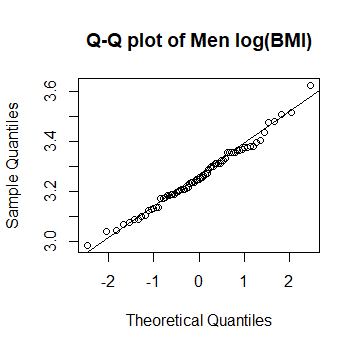
\includegraphics[scale=0.9]{root/qqmenlog.png}
    \caption{Q-Q plot of logged BMI scores for men}
    \label{menqq}
    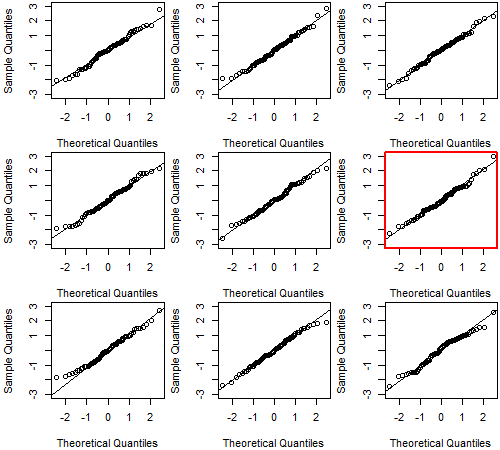
\includegraphics[scale=0.9]{root/menwally.png}
    \caption{Wally plot of men}
    \label{wallymen}
\end{figure}
As before it is possible to say that the data are normally distributed. \\
\begin{figure}[h!]
    \centering
    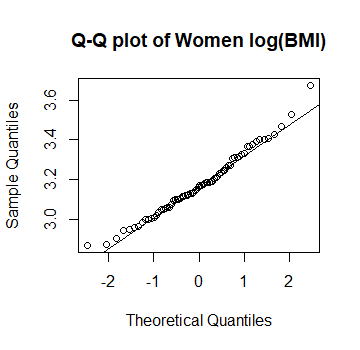
\includegraphics[scale=0.9]{root/qqwomenlog.png}
    \caption{Q-Q plot of logged BMI scores for women}
    \label{womenqq}
    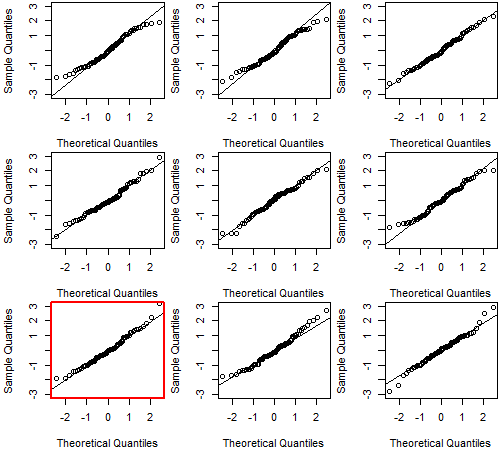
\includegraphics[scale=0.9]{root/wallywomen.png}
    \caption{Wally plot of women}
    \label{wallywomen}
\end{figure}
Even for the females it is hard to find back the plot, thus they are normally distributed. \\
\newpage
The parameters of the models are:
\begin{table}[h]
\centering
\begin{tabular}{|c||c|c|}
  \hline
 & \parbox{1.5cm}{\textbf{Sample mean}} & \parbox{1.5cm}{\textbf{Sample std. dev.}} \\
  \hline
  \hline
Women & 3.1741 & 0.1599   \\ 
  \hline
Men & 3.2605 & 0.1240   \\ 
  \hline
\end{tabular}
\caption{Estimates of mean and standard deviation}
\label{Table3}
\end{table}

\subsubsection{j)}
The $95\%$ CI for the mean have been calculated and following what was already done in section g the $95\%$ CI for the median have been found:
\begin{table}[h]
\centering
\begin{tabular}{|c||c|c|}
  \hline
\parbox{1.5cm}& \parbox{1.5cm}{\textbf{Lower bound of CI}} & \parbox{1.5cm}{\textbf{Upper bound of CI}}  \\ 
  \hline
  \hline
Women & 23.0237 & 24.8204 \\ 
  \hline
Men & 25.3221 & 26.8294 \\
\hline
\end{tabular}
\caption{Confidence intervals for the medians}
\label{Table4}
\end{table}

\subsubsection{k)}
The hypothesis that is going to be tested is that the difference between $\mu_{log\_men}$ and $\mu_{log\_women}$ is zero. 
\[ H_0:\mu_{log\_men}-\mu_{log\_women} = 0\]  
\[ H_1:\mu_{log\_men}-\mu_{log\_women} \ne 0\]  
Using the $95\%$ CI we can say that $\alpha = 0.05$, this represents the probability of the assumption being wrong.
The formula for the test statistics is:
\[ t_{obs} = \frac{(\overline{x_1}-\overline{x_2})-\delta_0}{\sqrt{s_1^2/n_1+s_2^2/n_2}}    \]
The distribution of test statistics is:
\[ T = \frac{(\overline{X_1}-\overline{X_2})-\delta_0}{\sqrt{S_1^2/n_1+S_2^2/n_2}}    \]
With $v$ degrees of freedom:
\[ v = \frac{(\frac{s_1^2}{n_1}+\frac{s_2^2}{n_2})^2}{\frac{(s_1^2/n_1)^2}{n_1-1}+\frac{(s_2^2/n_2)^2}{n_2-1}}          \]
The p-value is found using: 
\[  p-value = 2P(T>|t_{obs}|) \]
The found p-value is: $0.000382$ \\
It is possible to state that since the p-value is much smaller than $\alpha$ and it is very small in general we reject the hypothesis where the two genders have the same BMI (high evidence against it so reject $H_0$), thus there is a difference between the females BMI and males one ($H_1$). Comparing the results with the given R code we notice that our CIs are positive, but this depends the order in which the samples for the Welch test are chosen.

\subsubsection{l)}
The same conclusion could have definitely been drown from just the CIs. Using remark 3.59 from the text-book. \\ "In the case of two independent variables with added CIs we can say that: \\
when the two CIs do not overlap the two groups are significantly different." \\
And this is our case, see table \ref{Table4}.


\subsection{Correlation}

\subsubsection{m)}
In order to compute the correlation we need to use the covariance, found like this:
\[ s_{xy} = \frac{1}{n-1} \sum_{i=1}^{n} (x_i-\overline{x})(y_i-\overline{y}) \]
and use it in the correlation formula, that is:
\[ r=\frac{1}{n-1}\sum_{i=1}^{n} \left( \frac{x_i-\overline{x}}{s_x} \right) \left( \frac{y_i-\overline{y}}{s_y} \right)=\frac{s_{xy}}{s_x \cdot s_y}\]
In particular the correlation formula between BMI and weight is:
\[ r=\frac{1}{n-1}\sum_{i=1}^{n} \left( \frac{x_i-\overline{x}}{s_x} \right) \left( \frac{y_i-\overline{y}}{s_y} \right)=\frac{s_{xy}}{s_x \cdot s_y}=\frac{48.27}{15.21 \cdot 3.83}=0.83 \]
With the correlations between BMI and weight, BMI and fast food, weight and fast food the scatter plots have been made. The results for correlations of BMI and fast food and fast food and weight have a low value of correlations thus they are not included here because the representation is not significant. The correlation between BMI and weight is a clear indication that as people's weight increases also their weight does the same.
\begin{figure}[h]
    \centering
    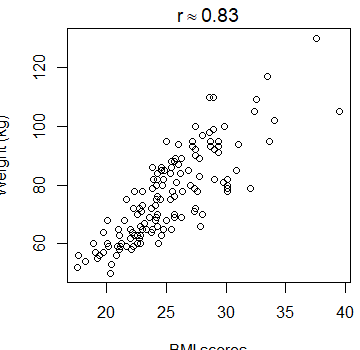
\includegraphics[scale=1]{root/Scatter.png}
    \caption{Scatter plot of BMI vs. weight}
    \label{scatter}
\end{figure}
We can see that the trend is positive and there is a high level of linear relation between these two as we could expect.
